%% Copyright 2007, 2008, 2009 Elsevier Ltd
%% 
%% 
%% This file is part of the 'Elsarticle Bundle'.
%% ---------------------------------------------
%% 
%% It may be distributed under the conditions of the LaTeX Project Public
%% License, either version 1.2 of this license or (at your option) any
%% later version.  The latest version of this license is in
%%    http://www.latex-project.org/lppl.txt
%% and version 1.2 or later is part of all distributions of LaTeX
%% version 1999/12/01 or later.
%% 
%% The list of all files belonging to the 'Elsarticle Bundle' is
%% given in the file `manifest.txt'.
%% 
%% Template article for Elsevier's document class `elsarticle'
%% with harvard style bibliographic references
%% SP 2008/03/01

\documentclass[preprint,12pt,authoryear]{elsarticle}

%% Use the option review to obtain double line spacing
%% \documentclass[authoryear,preprint,review,12pt]{elsarticle}

%% Use the options 1p,twocolumn; 3p; 3p,twocolumn; 5p; or 5p,twocolumn
%% for a journal layout:
%% \documentclass[final,1p,times,authoryear]{elsarticle}
%% \documentclass[final,1p,times,twocolumn,authoryear]{elsarticle}
%% \documentclass[final,3p,times,authoryear]{elsarticle}
%% \documentclass[final,3p,times,twocolumn,authoryear]{elsarticle}
%% \documentclass[final,5p,times,authoryear]{elsarticle}
%% \documentclass[final,5p,times,twocolumn,authoryear]{elsarticle}

%% For including figures, graphicx.sty has been loaded in
%% elsarticle.cls. If you prefer to use the old commands
%% please give \usepackage{epsfig}

%% The amssymb package provides various useful mathematical symbols
\usepackage{amssymb}
%% The amsthm package provides extended theorem environments
%% \usepackage{amsthm}
\usepackage{amsmath}
\usepackage{amssymb}
\usepackage{multirow}
\usepackage{alltt}
%\usepackage{cite}
\usepackage{booktabs}
\usepackage{float}
%\usepackage{natlib}
\usepackage{filecontents}
%\usepackage[style=authoryear-comp,firstinits=true]{biblatex}
%\usepackage{biblatex}


%% The lineno packages adds line numbers. Start line numbering with
%% \begin{linenumbers}, end it with \end{linenumbers}. Or switch it on
%% for the whole article with \linenumbers.
%% \usepackage{lineno}



%\begin{filecontents}{bibtest.bib}
%@article{Steinhubl:2008el,
%author = {Steinhubl, Steven R},
%title = {{Why Have Antioxidants Failed in Clinical Trials?}},
%journal = {The American Journal of Cardiology},
%year = {2008},
%volume = {101},
%number = {10},
%note    = {doi: \url{ doi:10.1016/j.amjcard.2008.02.003 }},
%pages = {S14--S19},
%month = may
%}
%
%\end{filecontents}


%\addbibresource{bibtest.bib}
\nocite{*}

%author = {Steinhubl, Steven R},
%title = {{Why Have Antioxidants Failed in Clinical Trials?}},
%journal = {The American Journal of Cardiology},
%year = {2008},
%volume = {101},
%number = {10},
%note    = {doi: \url{ doi:10.1016/j.amjcard.2008.02.003 }},
%pages = {S14--S19},
%month = may






\journal{Journal of Theoretical Biology}

\begin{document}
\bibliographystyle{elsarticle-harv} 

\newcommand{\inquotes}[1] { ``{#1}''}

\begin{frontmatter}

%% Title, authors and addresses

%% use the tnoteref command within \title for footnotes;
%% use the tnotetext command for theassociated footnote;
%% use the fnref command within \author or \address for footnotes;
%% use the fntext command for theassociated footnote;
%% use the corref command within \author for corresponding author footnotes;
%% use the cortext command for theassociated footnote;
%% use the ead command for the email address,
%% and the form \ead[url] for the home page:
%% \title{Title\tnoteref{label1}}
%% \tnotetext[label1]{}
%% \author{Name\corref{cor1}\fnref{label2}}
%% \ead{email address}
%% \ead[url]{home page}
%% \fntext[label2]{}
%% \cortext[cor1]{}
%% \address{Address\fnref{label3}}
%% \fntext[label3]{}



\title{Why antioxidant therapies have failed in clinical trials}


%% use optional labels to link authors explicitly to addresses:
%% \author[label1,label2]{}
%% \address[label1]{}
%% \address[label2]{}

\author{Adrian Davies and Alan Holt}

\address{}

\begin{abstract}

In spite of considerable research, and many clinical trials involving thousands of patients, there is a conspicuous lack of antioxidant therapies available. In this paper we present results for the interaction and neutralization of a free radical species. We adopt two modeling techniques, one based upon Gillespie’s Stochastic Simulation Algorithm and one based upon a discrete Markov chain. An advantage of these models is that they incorporate the number of molecules present per unit volume, and with the Markov chain model, the relative dimensions of these molecules. By means of these models we question the basis of antioxidant therapies based trapping or scavenging of reactive species. We demonstrate the extraordinary capacity of the enzymatic antioxidant defenses relative to non-enzymatic defenses. We conclude that, if the concentration of an non-enzymatic antioxidant is too low there is little chance of collision and interaction with a free radical species. Furthermore, if the rate of reaction between the free radical and the non-enzymatic antioxidant is below a necessary threshold then the effect of an antioxidant will be dwarfed by the free radical defense systems naturally present. As such, we suggest that failure of most antioxidant therapies in clinical trials, is to be expected.

%
%needs to be present at
%a sufficiently high concentration to give a reasonable chance
%of interaction between the antioxidant,
%rather than with other components of the cell
%
% within the scope of these models we suggest that there is limited therapeutic potential for non-enzymatic antioxidants that function by trapping or scavenging free radical species, and that the failure of many putative antioxidant compounds to demonstrate a therapeutic effect is to be expected.
%
%
%

\end{abstract}

\begin{keyword}
Antioxidant, Free Radical, ROS, Gillespie, Markov Model
%% keywords here, in the form: keyword \sep keyword

%% PACS codes here, in the form: \PACS code \sep code

%% MSC codes here, in the form: \MSC code \sep code
%% or \MSC[2008] code \sep code (2000 is the default)

\end{keyword}

\end{frontmatter}

%% \linenumbers

%% main text
\section{Introduction}
\label{}

The free radical theory of ageing, \citet{Harman:1956wu}, put forward the hypothesis that
free radicals, usually reactive oxygen species, generated as a by product of respiration are a causal
factor in the process of ageing. This is based on the supposition that free radicals are highly reactive
and are a cause of continual and cumulative damage to cellular protein, lipid, and
DNA (the soma). This damage, unless repaired, will lead to a progressive
deterioration of cellular function. Cumulative damage by free radicals has been associated
with many diseases, notably age related neurodegenerative conditions such as
Alzheimer's. This is, in part, because the brain has a high metabolic demand and a
subsequently high oxygen demand, while being essentially post-mitotic, \citet{Cobley:2018kt}.  
While it is well established that antioxidants like ascorbic acid can neutralize many free radical
species, the use of antioxidants in clinical trials has shown them to be predominately ineffective, see \citet{Steinhubl:2008el}. 
The chemistry of the free radical trapping proporties of vitamin C (ascorbic acid) are well documented, 
however, just because the chemistry is plausible, it does not necessitate that it occurs \emph{in vivo} or 
that it is effective. Ascorbic acid can be taken orally but there is negligable absorbtion at doses greater than 500mg (about five oranges worth) at which point it will increase the plasma concentration to a steady state of 80 micromolar, \citet{Padayatty:2003}. The cells and tissues of a typical and well nourished person will already contain ascorbic acid at 1-4 millimolar. 
One would assume that, if ascorbic acid is already present at a high concentration and provided an effective defense against free radicals, but would be even more effective at a slightly higher concentration, that this would have occured.

To address the question of the effectiveness of antioxidants, the process of oxidative damage and the mechanisms to avoid it can be reduced to a number of basic processes. Namely, the generation of free radicals and their subsequent neutralization by specific enzymatic means, neutralization by non-enzymatic antioxidants, or damage to the soma. This is shown schematically in Fig \ref{fig:g1}.




\begin{figure}
\begin{center}
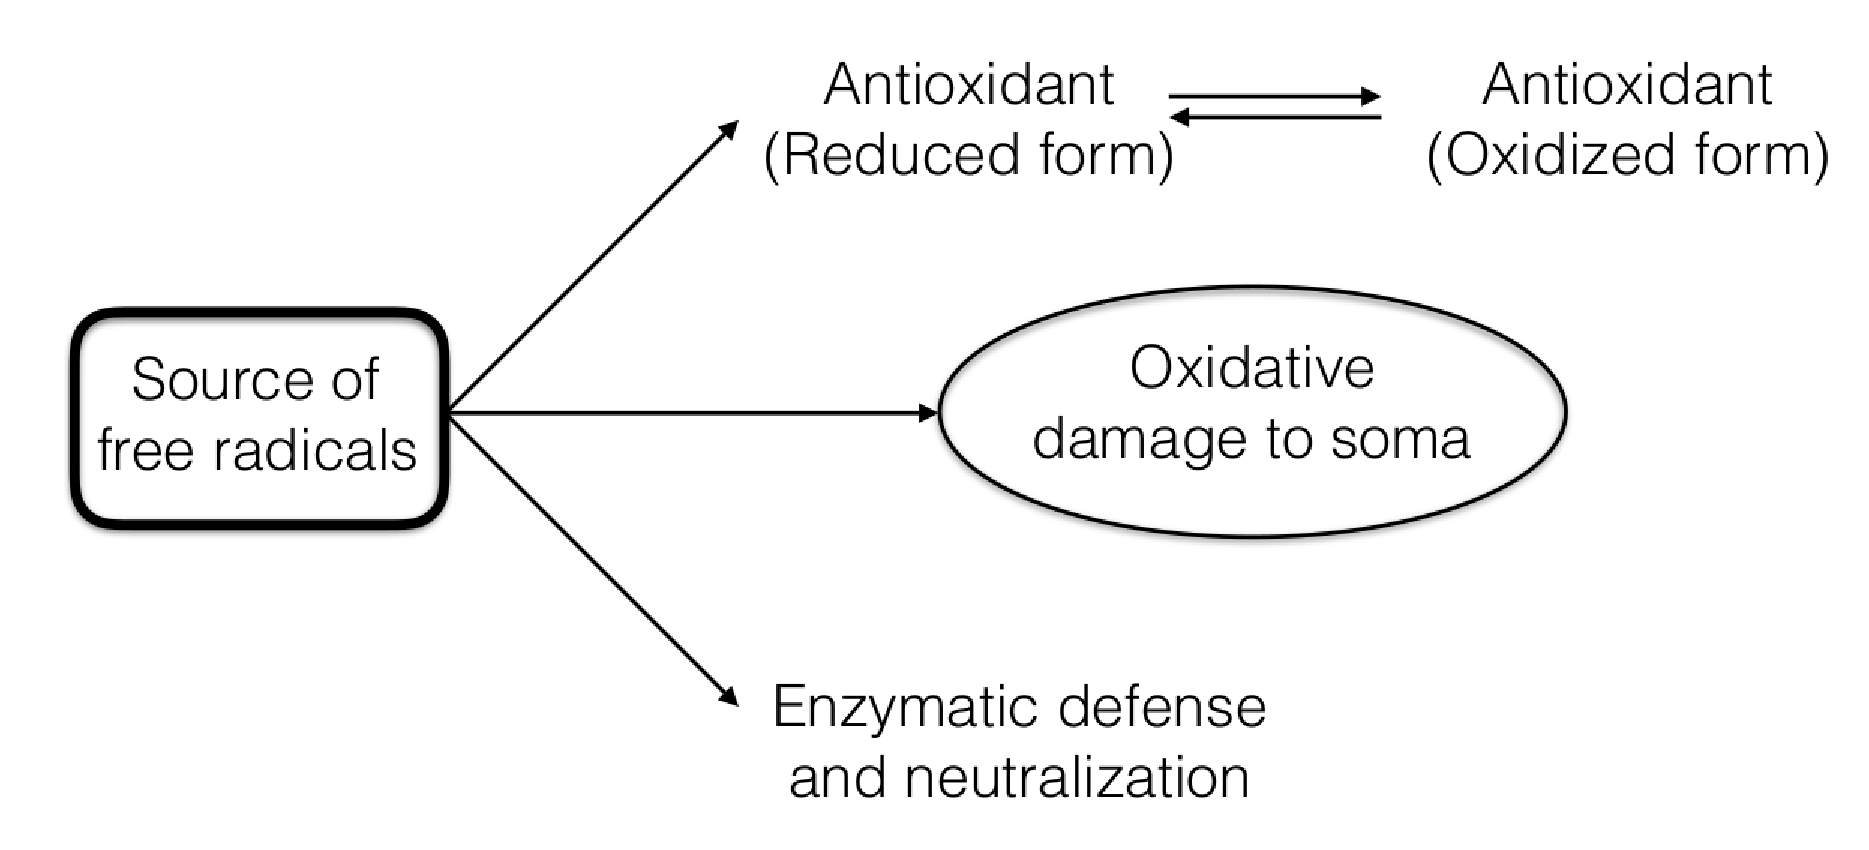
\includegraphics[width=0.8\textwidth]{Figure1.eps}
\end{center}
\caption{\label{fig:g1} Generalized scheme for the interactions of free radicals. After their generation
free radical species can be neutralized by scavenging antioxidants, enzymatic defenses, or
interact with and damage components of the cell.}
\end{figure}

In this paper we adopt two modeling techniques, namely Gillespie's Stochastic Simulation Algorithm
(using Kinetiscope) and a discrete Markov chain. The two models yield comparable results.


\section{Model of Free Radical Interactions}

In this section we develop a model of free radical interactions 
by imagining a highly simplified organelle, it functions much like a
mitochondrion. The parameters for the number and size of molecules in the cell were taken from
the \emph{By the numbers} website\footnote{http://bionumbers.hms.harvard.edu/}
and associated publications, \citet{Milo:2015uq}. A typical human cell such as a fibroblast has a volume of $2,000 \mu m^3$, and the mass of mitochondria is 20-25\% of the total cell volume.
As such, we defined the volume of the imaginary organelle as $400 \mu m^3$ and assigned arbitrary values to the cell 
contents, that is, $1 \times 10^9$ protein molecules, $1 \times 10^{10}$
molecules of water, and $1 \times 10^8$ molecules of a non-enzymatic antioxidant, \citet{bergsten:1989}.
Of the protein present $3 \times 10^7$ molecules (3\%) are an enzymatic antioxidant.
For interaction with the free radical the initial rate constant assumed for the non-enzymatic antioxidant was
$3 \times 10^5 M^{-1} s^{-1}$, and for the enzymatic antioxidant it was $1 \times 10^ 9 M^{-1} s^{-1}$. 
The high value for the enzymatic antioxidant is due to the fact that superoxide dismutase is an unusual enzyme and operates far faster than most enzymes, and may be as fast as it is theoretically possible.

%Kinetiscope is based
%on stochastic algorithms, \citet{Gillespie:2007bx}, instead of integration of differential
%equations.

The  modeling software used was Kinetiscope from Columbia Hill Technical
Consulting\footnote{http://www.hinsberg.net/kinetiscope/license.html}. 
The algorithm is based upon Gillespie's Stochastic Simulation Algorithm,  \citet{Gillespie:2007bx}. 
The algorithm calculates the probabilities of all reactions in the system. 
For each iteration, reactions are selected at random, weighted by their probabilities which are 
derived from their respective rate constants.

The values used were loosely based on the rate constants for the reactions of superoxide with glutatione, \citet{Winterbourn:2016cu}, 
with ascorbic acid, \citet{Buettner:1996vo},
and superoxide dismutase, \citet{Milgrom:2016iw}. The rate for damage to the soma was set at $300 M^{-1} s^{-1}$ based of the rate of superoxide
interaction with methionine protein residues, \citet{Davies:2016kz}.
An arbitrary rate of free radical generation of $1 \times 10^{-6} s^{-1}$ was selected to give a
measurable rate of protein oxidation in a reasonable time span. The actual rate of
generation of free radicals, specifically superoxide, by mitochondria has not been accurately determined, \cite{Murphy:2009jy}. 
This is, in part, due to the high catalytic rate of enzymes such as superoxide dismutase and catalase which maintain a low steady state level of superoxide and hydrogen peroxide.

In the absence of enzymatic antioxidants or non-enzymatic antioxidants the rate of damage to the protein was, as would be
expected, proportional to the rate of generation of free radicals (not shown).
Enzymes involved in the defence against free radical damage such as superoxide dismutase and catalase have extremely high catalytic rates, and are some of the most abundant proteins present in the cell ($\sim 1-3$\% from PaxDb:
Protein Abundance Database\footnote{https://pax-db.org}). If the concentration of the enzymatic antioxidant is
set to 3\% of the total protein and the $k_{cat}/K_M$ is varied, it can be seen (see Fig \ref{fig:g2a}) that
in order to reduce the rate of damage to the soma (protein in this model) to a negligible level a $k_{cat}/K_M$ of
$3 \times 10^8 M^{-1} s^{-1}$ to $1 \times 10^9 M^{-1} s^{-1}$ is required.
Coincidentally this is close to the observed
$k_{cat}/K_M$ of enzymes such as catalase and superoxide dismutase, \citet{Milgrom:2016iw}. Conversely if we define the $k_{cat}/K_M$ of
the enzymatic antioxidant as $1 \times 10^9 M^{-1} s^{-1}$ and vary the concentration of the enzymatic antioxidant, the
concentration at which there is negligible oxidative damage to the soma is at
0.3-1\% of the total protein. This is reasonably close to the concentration of enzymes such as catalase and superoxide dismutase
at 1-3\% (Fig \ref{fig:g2b}).



%\begin{figure}[top]
\begin{figure}
\begin{center}
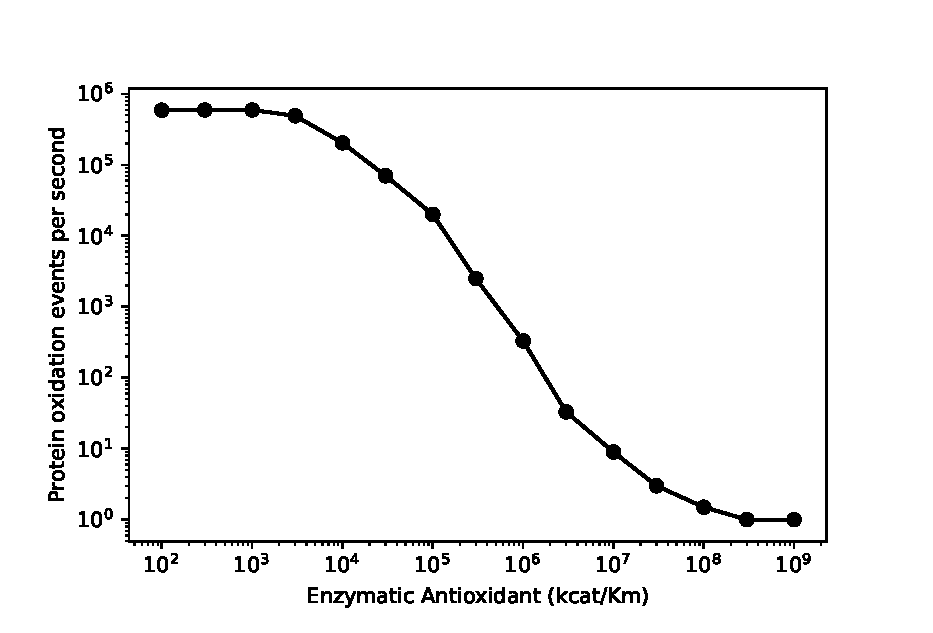
\includegraphics[width=0.8\textwidth]{Fig2A.eps}
\end{center}
\caption{\label{fig:g2a} 
Effect of variation in the amount of enzymatic antioxidant.
To inhibit the rate of oxidation of cellular protein the enzymatic antioxidant has to be present at 
$10^8$ molecules per cell or greater.
}
\end{figure}

\begin{figure}
\begin{center}
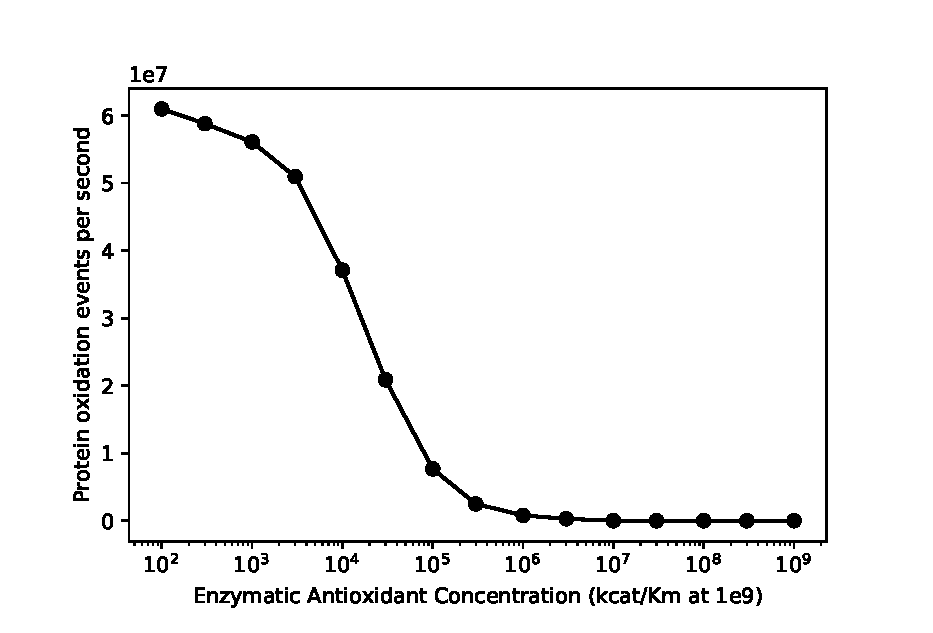
\includegraphics[width=0.8\textwidth]{Fig2B.eps}
\end{center}
\caption{\label{fig:g2b} The assigned rate constant for the reaction of enzymatic antioxidant with the free radical species can be varied. If the number of molecules per organelle is defined as $10^8$, then a $k_{cat}/K_M$ greater than  $10^7 M^{-1} s^{-1}$ is necessary. For reference the $k_{cat}/K_M$ of superoxide dismutase is $10^9 M^{-1} s^{-1}$}
\end{figure}



In order to be effective as an antioxidant, it is necessary to be
present at a relatively high concentration and to have a high forward rate constant ($k_{cat}/K_M$).
If a non-enzymatic antioxidant is added to the system at a high concentration
($1 \times 10^8$ molecules per cell) with a moderate $k_{cat}/K_M \approx 3 \times 10^5 M^{-1} s^{-1}$, in the absence of any
enzymatic antioxidant, it can be seen that it can function as an antioxidant for a short while (see Fig \ref{fig:g3}).
However, in the absence of a mechanism for the efficient regeneration of the
reduced form from the oxidized form, the antioxidant is rapidly depleted.


\begin{figure}
\begin{center}
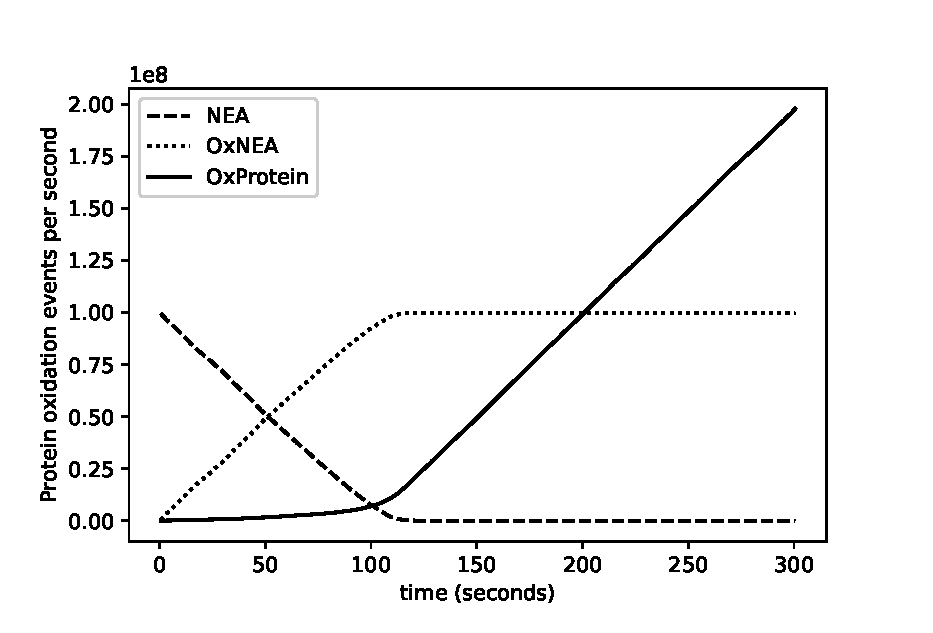
\includegraphics[width=0.8\textwidth]{Fig3.eps}
\end{center}
\caption{\label{fig:g3} Rapid depletion of a non-regenerating non-enzymatic antioxidant, with accumulation of the
oxidized form. When the store of the non-enzymatic antioxidant is exhausted there is rapid oxidation of
the cellular proteins.}
\end{figure}

These results indicate that, in comparson to endogenous antioxidants, non-enzymatic antioxidant are relatively ineffective at ameliorating oxidative damage from free radicals.
This is contrary to the conventional wisdom that exogenous antioxidants can reduce free radical damage, as such, we desired confirmation of this result. Thus, we developed a
second model based upon a discrete time Markov chain which we describe in  Section \ref{sec:mm} below.

\section{Markov Chain}
\label{sec:mm}

In this section we describe a discrete time Markov chain to model the
trajectory of a free radical within a cell. The cell in this model is comprised
of water molecules, protein molecules, enzymatic antioxidants, and non-enzymatic
antioxidants as previously defined. We further assume that there is a steady rate of free radical production.
During each time interval a free radical encounters either a water molecule, a
protein, an enzymatic antioxidant, or a non-enzymatic antioxidant.
We consider the trajectory of a free radical within a cell and its
likelihood of an encounter with each of the above components.
These likelihoods are governed by the relative abundance of each
component in the cell and their relative size.
Unlike the previous model our Markov model takes into account the relative volume occupied (size and number) of the molecules 
involved. Water, for example, is the most abundant molecule but is considerably smaller than a protein molecule.



An encounter with a water molecule (which we call state $w$)
has no effect on the free radical which  continues on its trajectory into
the next time interval (and, consequently, the next state).
The probability of an encounter with a water molecule $p(w)$ is derived from the ratio
of water and the total amount of matter in the cell, thus:
\begin{equation}
p(w) = \frac{m_{w} v_{w}} {M_{total}}
\end{equation}

We compute the total matter $M_{total}$ in the cell as:
\begin{equation}
M_{total} = m_{w} v_{w} + m_{prot} v_{prot} + m_{ea} v_{ea} + m_{nea} v_{nea}
\end{equation}

{\parindent0pt
where $m_{w}$, $m_{prot}$, $m_{ea}$ and $m_{nea}$ are the number of molecules of water, protein, enzymatic antioxidant, and non-enzymatic antioxidant, respectively.
Likewise, $v_{w}$, $v_{prot}$, $v_{ea}$ and $v_{nea}$ are the respective volumes for water, protein, enzymatic antioxidant, and non-enzymatic antioxidant.
}


The probability of an encounter with a protein is derived from the ratio
of the amount of protein and the total amount of matter in the cell ($M_{total}$).  
However, the effect of an encounter
with a protein molecule can yield two different results. Either the encounter is
productive and the free radical reacts with the protein of the encounter is \emph{futile}
resulting in no reaction.
A productive encounter results in a neutralisation of the
free radical  and its trajectory is terminated.
A productive encounter is an \emph{absorbing} state.
We should point out that a \emph{productive} encounter of a free radical with 
protein results in cell damage and equates to oxidative damage.
If the encounter is futile the state is \emph{non-absorbing}
and the free radical continues on its trajectory into the next time interval.
Consequently, we have transition probabilities for each of the productive and futile states, namely,
$p(prot_a)$ and $p(prot_{na})$, respectively.
The fraction of futile encounters for the protein ($\varphi_{prot}$) is derived from \citet{barevan:2015uy}:
%
\begin{equation}
\varphi_{prot} = 1 - k_{prot}/\tilde{k}_1
\end{equation}

{\parindent0pt
where $k_{prot}$ is the $k_{cat}/K_M$  value for protein 
and $\tilde{k}_1$ is the diffusion limit rate constant. According to 
\citet{barevan:2015uy} $\tilde{k}_1$ is between $10^{9}$ and $10^{10} M^{-1}s^{-1}$.
The purpose of this paper we use $\tilde{k}_1 = 10^{10}$.
From Table \ref{tbl:molecules},  $k_{cat}/K_M = 300 M^{-1}s^{-1}$.
}



%
The probability $p(prot_a)$ is given by:
%
\begin{equation}
p(prot_a) =  
\frac{ (1-\varphi_{prot}) m_{prot} v_{prot} } { M_{total } }
\end{equation}

The probability $p(prot_{na})$ is given by:
%
\begin{equation}
p(prot_{na}) = 
\frac{ \varphi_{prot} m_{prot} v_{prot} } { M_{total}  }
\end{equation}

As with protein molecules,
we model an encounter with enzymatic antioxidant as productive and futile encounter states to reflect the effect
on the free radical, that is, the encounter either results in a reaction or no reaction with the enzymatic antioxidant, respectively.
With the enzymatic antioxidant (as well as the non-enzymatic antioxidant) a \emph{productive} encounter with a free radical
neutralizes it.
We use $ea_{a}$ to represent the productive encounter state and $ea_{na}$ to represent the futile encounter state.
State $ea_a$ is absorbing because
the trajectory of the free radical is terminated during the current time interval.
Conversely, the $ea_{na}$ state is non-absorbing as the free radical does not react
with the enzymatic antioxidant and its trajectory continues on into the next time interval.
The fraction of futile encounters for the enzymatic antioxidant is computed, thus:
%
\begin{equation}
\varphi_{ea} = 1 - k_{ea}/\tilde{k}_1
\end{equation}

The term $k_{ea}= 10^{9}$ is the $k_{cat}/K_M$  value for the enzymatic antioxidant (see Table \ref{tbl:molecules}).
The probability $p(ea_a)$ is given by:
%
\begin{equation}
p(ea_a) =  
\frac{(1-\varphi_{ea}) m_{ea} v_{ea}} {M_{total}}
\end{equation}


The probability $p(ea_{na})$ is given by:
\begin{equation}
p(ea_{na}) = 
\frac{ \varphi{ea}  m_{ea_{na}} v_{ea_{na}}} {M_{total}}
\end{equation}


Like the enzymatic antioxidant, a non-enzymatic antioxidant has a productive encounter 
state ($nea_{a}$) and a futile encounter state $nea_{na}$ which
are absorbing and non-absorbing, respectively.
Functionally, there is no difference between an enzymatic antioxidant or non-enzymatic antioxidant with rapid
regeneration, the main factor is the processing time, which can be
viewed as the equivalent of the forward rate constant. 
The fraction of futile  encounters with the  non-enzymatic antioxidant  is given by:
%
\begin{equation}
\varphi_{nea} = 1 - k_{nea}/\tilde{k}_1
\end{equation}

{\parindent0pt
where $k_{ea} = 10^{5}$ is the $k_{cat}/K_M$  value for the non-enzymatic antioxidant (Table \ref{tbl:molecules}).
%
%Based on the published rates of free radicals
%interaction with superoxide dismutase, catalase, glutathione,
%ascorbic acid, and protein it is evident that the rates are
%$k_{ea} \gg k_{nea} \gg k_{prot}$
%where $k_{nea}$ is the kcat value for non-enzymatic antioxidant
%(see Table \ref{tbl:molecules}).
%However, the rates of interaction and processing differ
%by orders of magnitude.
The probability $p(nea_{a})$ is given by:
}
%
%
\begin{equation}
p(nea_{a}) = 
\frac{\varphi_{nea} m_{nea_a} v_{nea_a}} {M_{total}}
\end{equation}

The probability $p(nea_{na})$ is given by:
%
\begin{equation}
p(nea_{na}) = 
\frac{(1-\varphi_{nea}) m_{nea_{na}} v_{nea_{na}}} {M_{total}}
\end{equation}

Table \ref{tbl:molecules} shows the values used to compute quantities of material in the cell along with their
corresponding $k_{cat}/K_M$ values (where applicable). These values are used to derive transition probabilities for
the transition matrix $\textbf{T}$ of the Markov model:

\begin{equation}
\textbf{T} = 
\begin{bmatrix}
p(w) & p(prot_a) & p(prot_{na}) & p(ea_a) & p(ea_{na}) & p(nea_a) & p(nea_{na})   \\
0         & 1         & 0         & 0         & 0     & 0       & 0           \\
p(w) & p(prot_a) & p(prot_{na}) & p(ea_a) & p(ea_{na}) & p(nea_a) & p(nea_{na})   \\
0         & 0         & 0         & 1         & 0     & 0       & 0           \\
p(w) & p(prot_a) & p(prot_{na}) & p(ea_a) & p(ea_{na}) & p(nea_a) & p(nea_{na})   \\
0         & 0         & 0         & 0         & 0     & 1       & 0           \\
p(w) & p(prot_a) & p(prot_{na}) & p(ea_a) & p(ea_{na}) & p(nea_a) & p(nea_{na})   \\
\end{bmatrix}
\end{equation}

The probability of the system being in state $i$ at time $k$ is $\pi_{i}^{k}$:

\begin{equation}
\pi = \pi \textbf{T}
\end{equation}

{\parindent0pt
where $\lim_{k\to\infty}\pi = \pi^{(k)}$. Without any loss of generality, we assume that
the initial state of system is an encounter with water, thus, the initial state is:
}
%
\begin{equation}
\pi^0 = 
\begin{bmatrix}
1         & 0         & 0     & 0         & 0     & 0       & 0           \\
\end{bmatrix}
\end{equation}



\begin{table}
\begin{center}
\begin{tabular*}{1.0\textwidth}{ @{\extracolsep{\fill}} l r r r }
\toprule
 & No. molecules & Vol. molecules & $k_{cat}/K_{M}$ \\
      &               & $nm^3$        & $M^{-1}s^{-1}$   \\
\midrule
Water                      & $1.3 \times 10 ^ {13}$ & 0.01  & NA \\
Protein                    & $1.0 \times 10 ^ 9$    & 65.40 & 300      \\
Enzymatic antioxidant      & $3.0 \times 10 ^ {7}$  & 65.40 & $1 \times 10^9$   \\
Non-enzymatic antioxidant  & $1.0 \times 10 ^ {8}$  & 1.00  &  $1 \times 10^5$   \\
\bottomrule
\end{tabular*}
\end{center}
\caption{Assigned values for the abundance, dimensions, and rate constants in the model}
\label{tbl:molecules}
\end{table}

\begin{figure}
\begin{center}
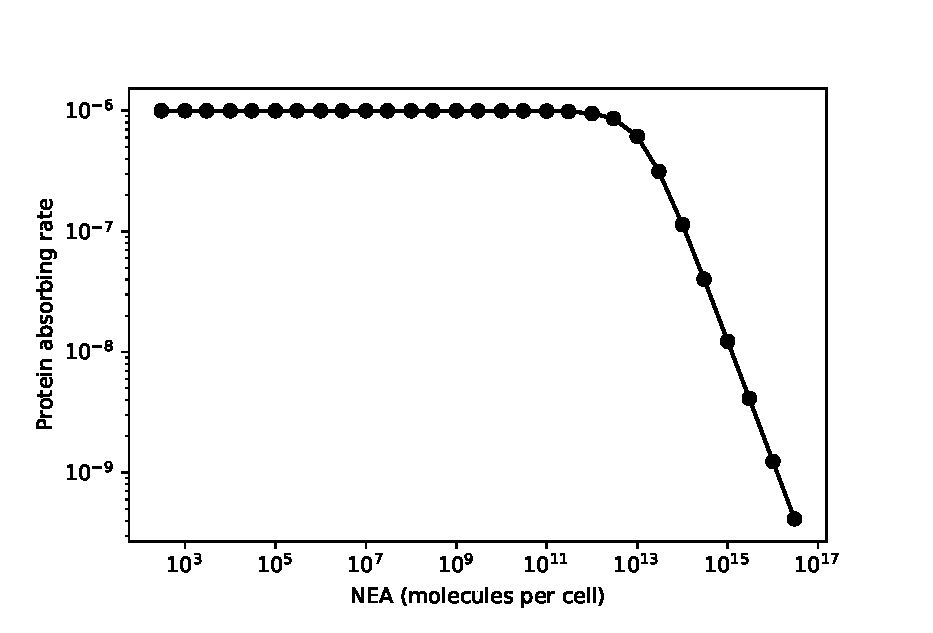
\includegraphics[width=0.8\textwidth]{Protein_absorbing.eps}
\end{center}
\caption{\label{fig:prot} Protein reaction.
It is apparent that, under the conditions specified in the model, that in order to reduce the rate of damage to protein by free radicals the non-enzymatic antioxidant would need to be present at physiologically unrealistic concentrations. A reduction in the rate of protein oxidation does not occur until the non-enzymatic antoxidant is present at greater than 
$10^{13}$ molecules per cell.
}
\end{figure}


We ran the model for varying levels of non-enzymatic antioxidant concentrations, 
namely, $10^3 \geq m_{nea} \geq 10^{17}$ and observed the effect on protein
reaction rates.
The rates of protein reaction (that is, damage to the cell) for various $m_{nea}$ 
are shown in Fig \ref{fig:prot}. 
Under these conditions it can be seen that the non-enzymatic antioxidant has 
a negligible effect for any realistic value of $m_{nea}$. 
While mechanistically different, the rate of neutralization of free radical species 
by enzymatic antioxidants is far greater than the rate of neutralization by 
non-enzymatic antioxidants, which in turn occurs at a much faster rate than damage 
to proteins by the free radical species, that is, $k_{ea} \gg k_{nea} \gg k_{prot}$.
Furthermore, these rates differ by several orders of magnitude. 
Molecules with a size of the order of molecules such as glutathione and ascorbic acid 
are relatively small compared to cell components such as protein. To be effective 
physical interaction between the free radical and the putative antioxidant is necessary, 
this interaction is limited by physical size and numerical presence.

%\begin{figure}
%\begin{center}
%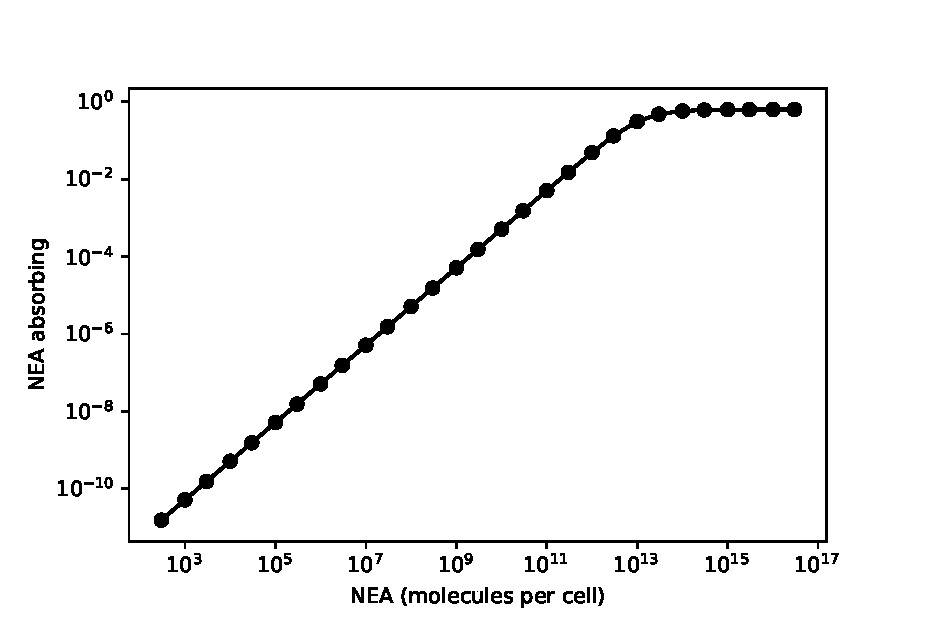
\includegraphics[width=0.8\textwidth]{NEA_absorbing.eps}
%\end{center}
%\caption{\label{fig:g4} To be an effective a non-enzymatic antioxidant with an assigned $k_{cat}/K_M$ of $3.0 \times 10 ^ {7}M^{-1} s^{-1}$ needs to be present at a high concentration, considerably in excess of a billion molecules per cell. }
%\end{figure}
%

\section{Conclusions}


In this paper we present two models of free radical interactions in a cell. The first employs
Gillespie’s Stochastic Simulation Algorithm from the stochastic modeling tool, Kinetiscope. The second
model is based upon a discrete Markov chain. 
These models are, purposely, highly abstracted and reductive because they are not intended to mimic or replicate an actual biological system. 
The purpose was to explore the parameters that most influence the potential interaction and termination of a free radical species. 
The models used different approaches but their results are in qualitative agreement.  


They illustrate that enzymes involved in defense against oxidative damage,
such as superoxide dismutase and catalase  are already extremely effective. At the
concentrations seen $in$ $vivo$ enzymatic antioxidants such as superoxide dismutase or catalase will essentially eliminate oxidative damage. This is not
surprising, to achieve the catalytic rates observed empirically, enzymes such as superoxide dismutase and catalase must have been subject to
strong selective pressure and as such are probably optimal in terms of catalytic rate and concentration. Non-enzymatic antioxidants such as glutathione or ascorbic acid have relatively modest rates of reaction with superoxide, in spite of the presumably identical
selective pressures that acted on the enzymatic antioxidants. Based on these results we would infer that defense against free radicals is
not a major role for these compounds.
The results also permit a number of conclusions to be made concerning the role of
therapeutic non-enzymatic antioxidants in the prevention of
oxidative damage to the soma:
\begin{enumerate}
\item
To be effective, a non-enzymatic antioxidant that operates by
trapping or scavenging free radicals, needs to be present at 
a sufficiently high concentration to give a reasonable chance 
of interaction between the antioxidant,
rather than with other components of the cell.
These high concentrations likely to be physiologically unrealistic.
\item
A potential free radical scavenging agent would also need to have a 
sufficiently high rate constant to effectively compete with the 
enzymatic defense system. Unless the rate of reaction is of the order of
$1 \times 10^7 M^{-1} s^{-1}$ or greater, they will have little 
effect on the rate of protein oxidation.
\item
There also needs to be an effective and efficient means of regenerating the
reduced form of the antioxidant from the oxidized form. Without a mechanism to
regenerate the reduced form of an antioxidant from the oxidized form an
exogenous antioxidant would be rapidly depleted. For a synthetic or 
non-endogenous compound it is unlikely a mechanism for this will be present.
\end{enumerate}

The models presented in this paper are limited in the number of parameters considered and assumes that the reactions take place in an aqueous environment. 
Non-enzymatic antioxidants may have utility in a lipid membrane environment. In lipids oxidative damage can propagate by means of a chain reaction.
Nevertheless, within the scope of these models we suggest that  therapeutic potential for non-enzymatic antioxidants that function by trapping 
or scavenging free radical species, is limited. 
In order to reduce the rate of damage to protein by free radicals the non-enzymatic antioxidant would need to be present at physiologically unrealistic concentrations. A reduction in the rate of protein oxidation does not occur until the non-enzymatic antoxidant is present at greater than
$10^{13}$ molecules per cell.
Therefore,  the failure of many putative antioxidant compounds to demonstrate a therapeutic effect is to be expected.






%% The Appendices part is started with the command \appendix;
%% appendix sections are then done as normal sections
%% \appendix

%% \section{}
%% \label{}

%% If you have bibdatabase file and want bibtex to generate the
%% bibitems, please use
%%
%%  \bibliographystyle{elsarticle-harv} 
%%  \bibliography{<your bibdatabase>}

%% else use the following coding to input the bibitems directly in the
%% TeX file.

%\bibliography{refs}
\section{References}



\begin{thebibliography}{00}

% \bibitem[Author(year)]{label}
%% Text of bibliographic item

%\bibitem[ ()]{}

%{Vol 101},
%{Number 10},
%%{Month May}
%

\bibitem[Bar-Evan et al.(1996)] {barevan:2015uy}
Bar-Even A, Milo R, Noor E, and Tawfik DS,
(2015)
The Moderately Efficient Enzyme: Futile Encounters and Enzyme Floppiness.
{\em Biochemistry} 54(32), 
pp. 4969--4977
doi: 10.1021/acs.biochem.5b00621 

%\bibitem[Bergten et al.(1989)] {barevan:1989}
%Bergsten P, Amitai G, Kehrl J, Dhariwa K.R, Klein H.G and Levine M
%(1989)
%Millimolar Concentrations of Ascorbic Acid in Purified Human Mononuclear Leukocytes
%{ \em The Journal of Biological Chemistry },  265(5).
%pp. 258.-2587.

\bibitem[Bergsten et al.(1989)] {bergsten:1989}
Bergsten P, Amitai G, Kehrl J, Dhariwa K.R, Klein H.G and Levine M.
(1989)
Millimolar Concentrations of Ascorbic Acid in Purified Human Mononuclear Leukocytes
{ \em The Journal of Biological Chemistry },  265(5).
pp. 2584--2587.


\bibitem[Buettner and Jurkiewicz(1996)] {Buettner:1996vo}
Buettner, G R and Jurkiewicz, B A.
(1996)
Catalytic metals, ascorbate and free radicals: combinations to avoid.
{\em Radiation research}, 145(5).
pp. 532--541.
doi:10.2307/3579271.







\bibitem[Cobley et al.(2018)]  {Cobley:2018kt}
Cobley, James Nathan and Fiorello, Maria Luisa and Bailey, Damian Miles.
(2018).
13 reasons why the brain is susceptible to oxidative stress.
{ \em Redox biology},  15.
pp. 490--503.
doi:10.1016/j.redox.2018.01.008.
%month = jan


\bibitem[Davies(2016)] {Davies:2016kz}
Davies, Michael J.
(2016)
Protein oxidation and peroxidation.
{ \em Biochemical Journal}, 473(7).
pp. {805--825}.
doi:10.1042/BJ2015122.
%month = mar





\bibitem[Gillespie(2016)] {Gillespie:2007bx}
%@article{Gillespie:2007bx,
Gillespie, Daniel T.
(2007).
Stochastic Simulation of Chemical Kinetics.
{ \em Annual Review of Physical Chemistry},  58(1).
pp.  {35--55},
doi:10.1146/annurev.physchem.58.032806.104637.


\bibitem[Harman(2016)] {Harman:1956wu}
{Harman, D}.
(1956).
Aging: a theory based on free radical and radiation chemistry.
{\em Journal of Gerontology},  11(3).
pp. {298--300}.
doi:10.1093/geronj/11.3.298.
%month = jul

\bibitem[ Milgrom(2016)] {Milgrom:2016iw} 
Milgrom, Lionel R.
(2016).
Why Is Catalase So Fast? A Preliminary Network Hypothesis for the Rapid Enzyme-catalysed Decomposition of Hydrogen Peroxide.
{\em WATER journal}, 7.
pp. 129--146.
doi:10.14294/Water.2016.1.

\bibitem[ Milo and Phillips(2015)] {Milo:2015uq}
Milo, Ron and Phillips, Rob.
(2015).
Cell Biology by the Numbers.
{\em Garland Science }.
% dec

\bibitem[ Murphy(2009)] {Murphy:2009jy}
Murphy, Michael P.
(2009).
How mitochondria produce reactive oxygen species.
{ \em Biochemical Journal},  417(1).
pp. {1--13}.
doi:10.1042/BJ20081386.

\bibitem[ Steinhubl(2008)] {Steinhubl:2008el}  
%@article{Steinhubl:2008el,
Steinhubl, Steven R.
(2008).
Why Have Antioxidants Failed in Clinical Trials?
{\em The American Journal of Cardiology},  101(10).
pp. S14--S19.
doi:10.1016/j.amjcard.2008.02.003.


\bibitem[ Winterbourn(2016)] {Winterbourn:2016cu}
Winterbourn, Christine C.
(2016).
Revisiting the reactions of superoxide with glutathione and other thiols.
{ \em Archives of Biochemistry and Biophysics},  595.
pp. {68--71}.
doi:10.1016/j.abb.2015.11.028.

\bibitem[ Padayatty(2003)] {Padayatty:2003}
Padayatty, Sebastian J. .
(2003).
Vitamin C as an Antioxidant: Evaluation of Its Role in Disease Prevention.
{ \em Journal of the American College of Nutrition},  22.
pp. {18--35}.
doi:10.1080/07315724.2003.10719272.
%
\end{thebibliography}




\end{document}

\endinput
%%
%% End of file `elsarticle-template-harv.tex'.
